\documentclass{beamer}
%\usepackage[latin1]{inputenc}
%\usepackage{lmodern}
\usepackage{times}
\usepackage[T1]{fontenc}
\usepackage{graphicx}
\usepackage{bm}
\usepackage[small,labelformat=empty]{caption}
\usepackage{url}

\usetheme{Frankfurt}
%\usetheme{Warsaw}
\title[r0ket]{\\
{\small this is r0ket science}
}
\author[team r0ket]
{team r0ket <\url{team@badge.events.ccc.de}>}
\institute[CCC]{}
\date{2010-08-10 - Day 1 @ CCCamp11}

\begin{document}

{
%\usebackgroundtemplate{\includegraphics[width=\paperwidth]{bilder/behindthescreen.jpg}}
\begin{frame}
\thispagestyle{empty}
\titlepage
\end{frame}
}

\begin{frame}
\frametitle{Fahrplan}
\tableofcontents
\end{frame}

\setlength\fboxsep{5pt}
\setlength\fboxrule{0pt}

\section{Motivation}
  \begin{frame}{Other Badges}
  \begin{columns}
    \begin{column}{6cm}
        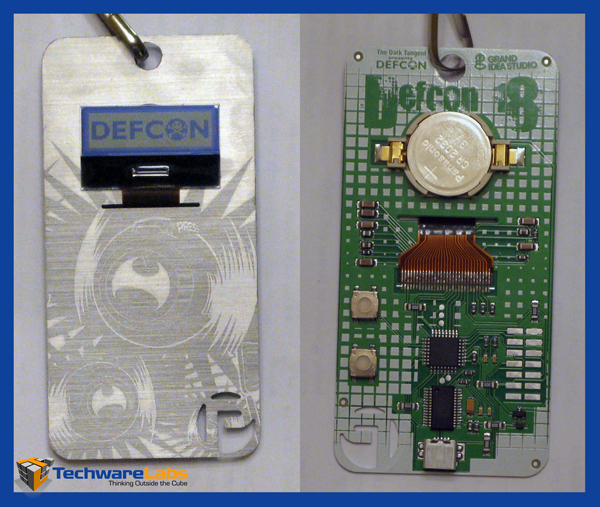
\includegraphics[height=4cm]{bilder/defcon1.jpg}\\
        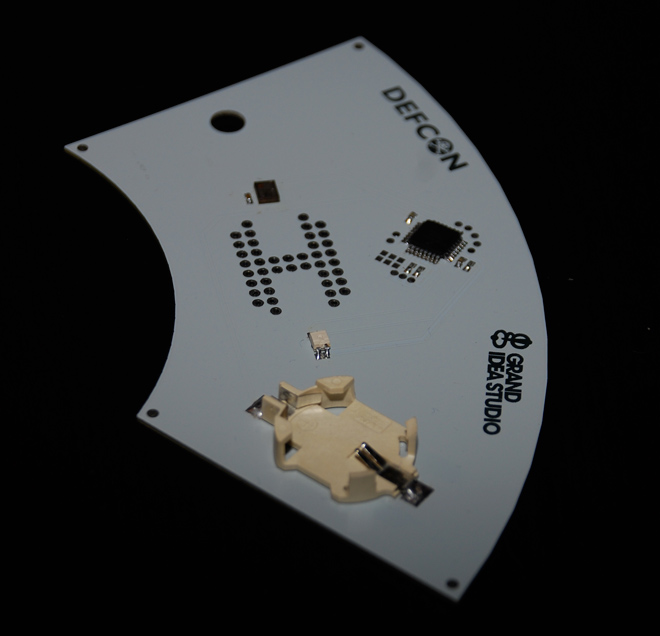
\includegraphics[height=4cm]{bilder/defcon2.jpg}
    \end{column}
    \begin{column}{6cm}
        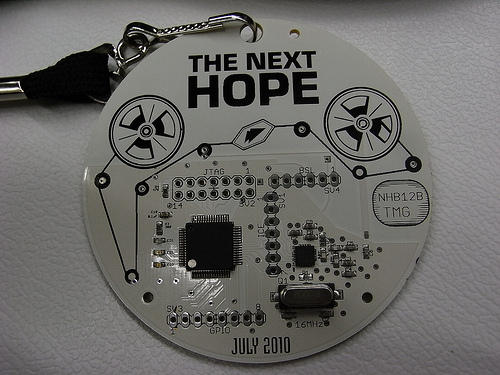
\includegraphics[height=4cm]{bilder/hope.jpg}\\
	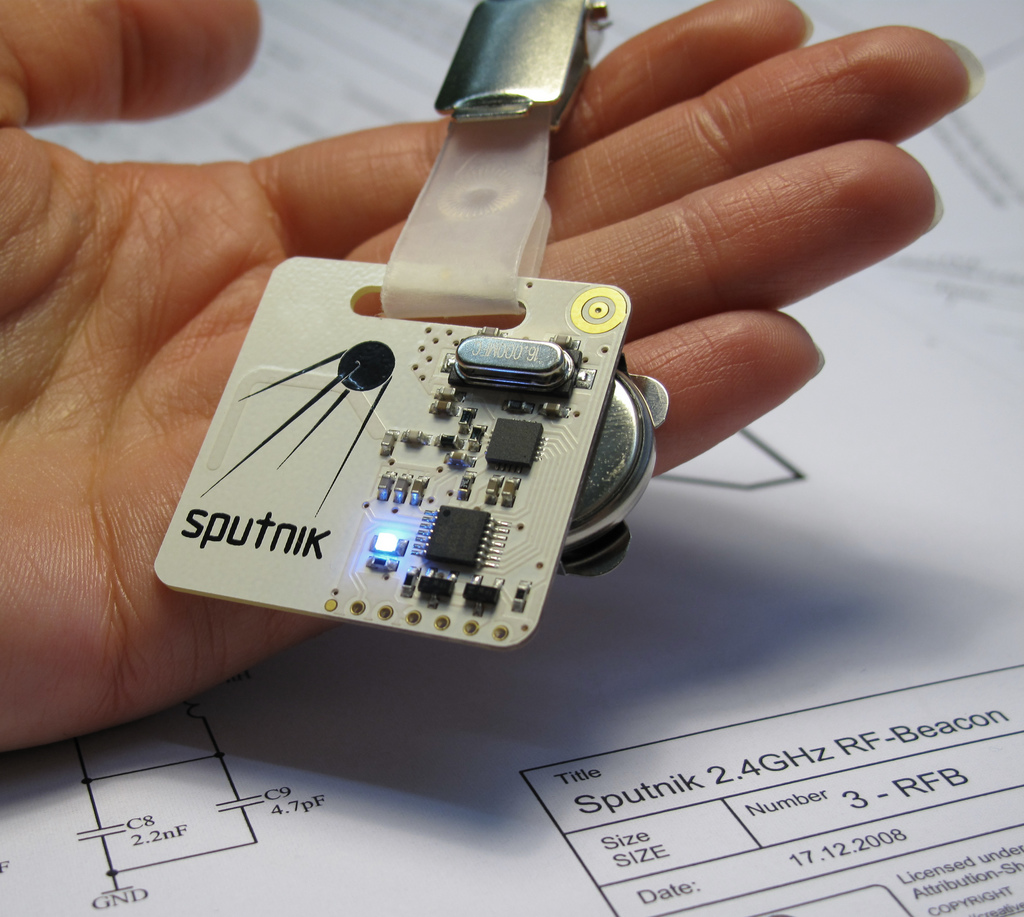
\includegraphics[height=4cm]{bilder/sputnik.jpg}
    \end{column}
  \end{columns}
  \end{frame}

\begin{frame}{Our first badge}
  \begin{columns}
    \begin{column}{6cm}
        \begin{itemize}
	    \item For the easter hegg 2010 in Munich.
	    \item AVR with 8kB program memory.
	    \item 100 kits soldered by participants.
	    \item Sold out in minutes.
	\end{itemize}
    \end{column}
    \begin{column}{6cm}
        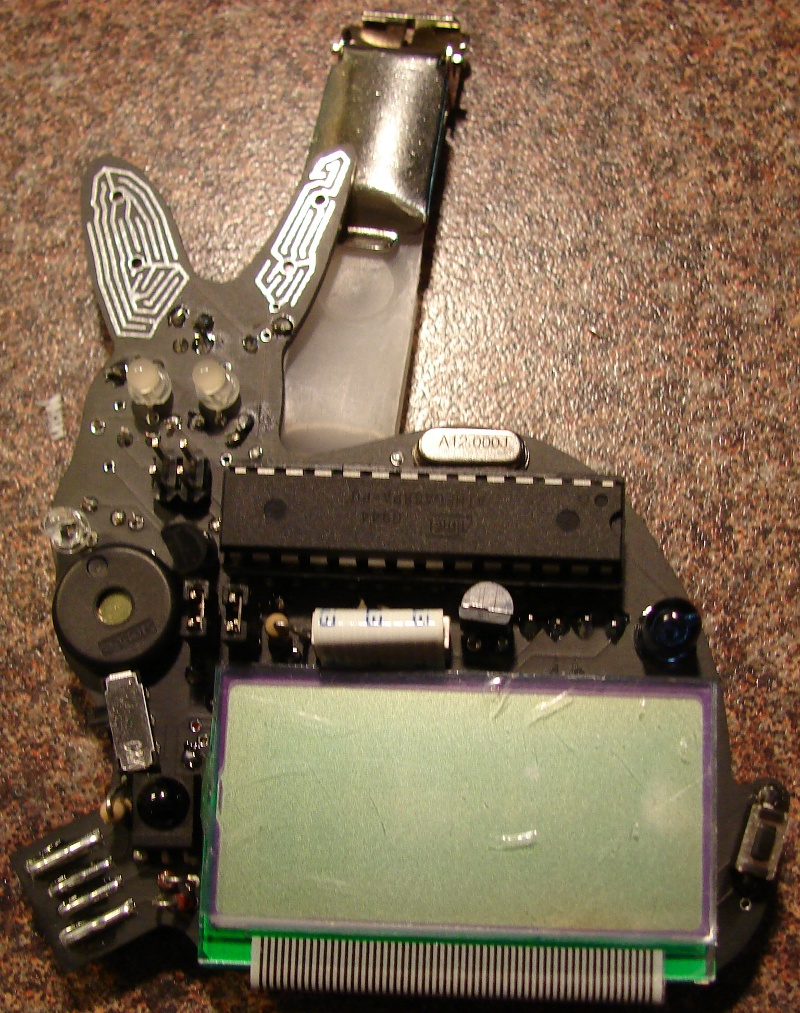
\includegraphics[height=4cm]{bilder/ehaserl.jpg}\\
    \end{column}
  \end{columns}
  \end{frame}
\begin{frame}{What happens after the event?}
	\begin{itemize}
		\item After the event most badges end up in the drawer.
		\item Coin cells are expensive, never at hand and always empty.
		\item Bigger batteries needed for a backlight.
	\end{itemize}
\end{frame}
\begin{frame}{Let's do it "right"}
	\begin{itemize}
		\item No more disposable batteries.
		\item Populated headers for extensions.
		\item Only controllers which are supported by gcc.
	\end{itemize}
\end{frame}
\section{Hardware}
\begin{frame}{Battery}
  \begin{columns}
    \begin{column}{6cm}
        \begin{itemize}
		\item The evil daystar has regular downtimes.
		\item Backlights need lots of power.
		\item Lithium is the only real option.
		\item A 600mAh battery powers a backlight for at least one day.
		\item Integrated charge controller is independend from the firmware.
	\end{itemize}
    \end{column}
    \begin{column}{6cm}
        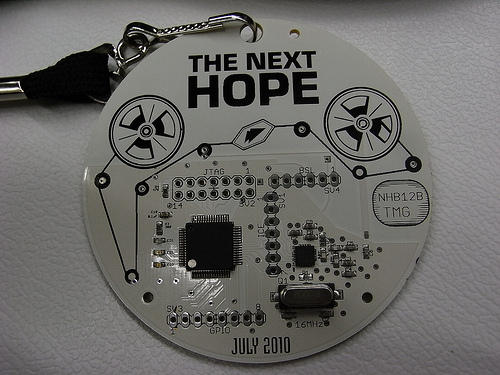
\includegraphics[height=4cm]{bilder/battery.jpg}
    \end{column}
  \end{columns}
\end{frame}
\begin{frame}{CPU}
  \begin{columns}
    \begin{column}{6cm}
        \begin{itemize}
		\item Today everyone does arduino.
		\item We wanted a more powerfull CPU
		\item NXP donated one of their ARM Cortex-M3 controllers to us.
		\item But: only 32kb flash...
	\end{itemize}
    \end{column}
    \begin{column}{6cm}
        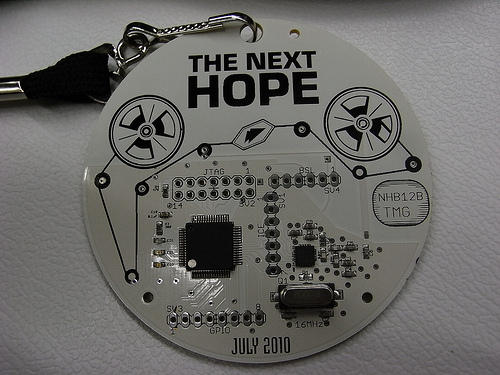
\includegraphics[height=4cm]{bilder/cpu.jpg}

        \includegraphics[height=4cm]{bilder/nxp.jpg}
    \end{column}
  \end{columns}
\end{frame}
\begin{frame}{LCD}
  \begin{columns}
    \begin{column}{6cm}
        \begin{itemize}
		\item Displays are more expensive than one might think
		\item But: Nokia made lots of them :)
		\item Found cheap and nice looking LCDs for old Nokia phones.
	\end{itemize}
    \end{column}
    \begin{column}{6cm}
%        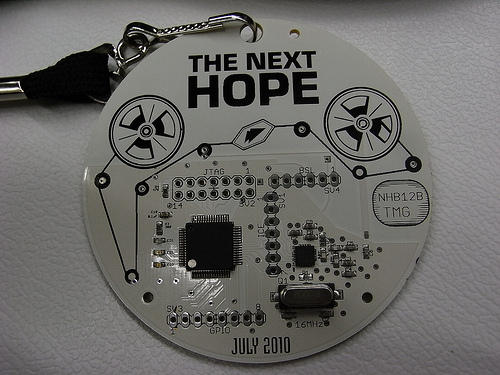
\includegraphics[height=4cm]{bilder/lcd.jpg}
	\includegraphics[width=6cm]{bilder/lcds.jpg}
    \end{column}
  \end{columns}
\end{frame}
\begin{frame}{Radio interface}
  \begin{columns}
    \begin{column}{6cm}
        \begin{itemize}
		\item At first a radio interface seemed to expensive.
		\item Milosch told us a good dealer for the chips OpenBeacon uses.
		\item The last protoype got a radio interface. It worked.
	\end{itemize}
    \end{column}
    \begin{column}{6cm}
        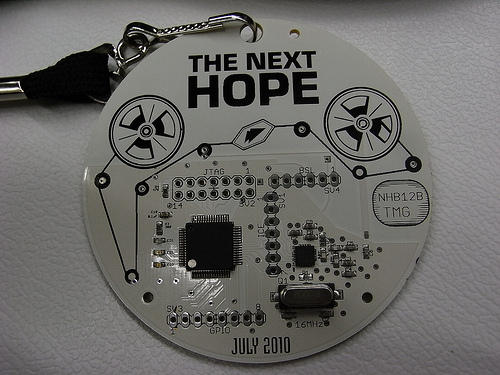
\includegraphics[height=4cm]{bilder/radio.jpg}
    \end{column}
  \end{columns}
\end{frame}
\begin{frame}{Modules}
  \begin{columns}
    \begin{column}{6cm}
        \begin{itemize}
		\item Modules extend the r0ket
		\item They can be combined with stackable headers
		\item Already there: Flame, Magnetometer, Flashlights
	\end{itemize}
    \end{column}
    \begin{column}{6cm}
        \includegraphics[height=4cm]{bilder/module.jpg}
    \end{column}
  \end{columns}
\end{frame}

\section{Production and Fuckups}
\begin{frame}{Design}
  \begin{columns}
    \begin{column}{6cm}
        \begin{itemize}
		\item First prototype was lame.
		\item Someone said: I'd like a rocket.
		\item We did r0ket :)
	\end{itemize}
    \end{column}
    \begin{column}{6cm}
        \includegraphics[height=8cm]{bilder/prototype.jpg}
    \end{column}
  \end{columns}
\end{frame}
\begin{frame}{PCBs}
  \begin{columns}
    \begin{column}{6cm}
        \begin{itemize}
		\item Ordered PCBs at a german company.
		\item Realized too late that they sub-contract to china.
		\item Colors are wrong, PCBs arrived late, panel was instable.
	\end{itemize}
    \end{column}
    \begin{column}{6cm}
	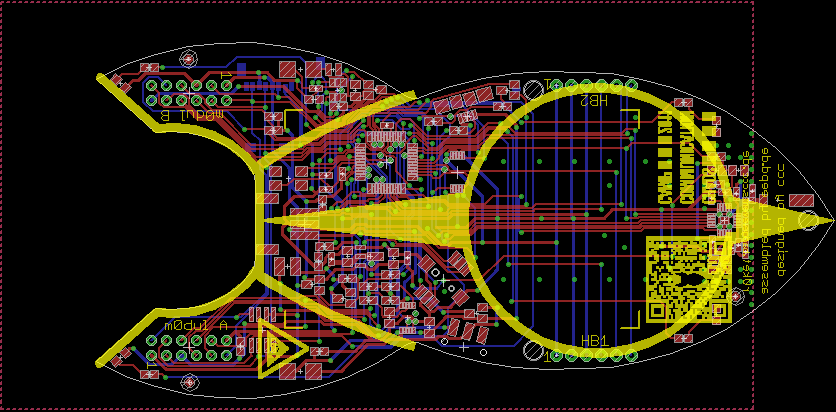
\includegraphics[width=6cm]{bilder/eagle.png}

        \includegraphics[width=6cm]{bilder/panel.jpg}
    \end{column}
  \end{columns}
\end{frame}
\begin{frame}{Production}
  \begin{columns}
    \begin{column}{6cm}
        \begin{itemize}
		\item Got a very good price at eepd.de
		\item Unbeatable: We got to test the first devices
		\item Only a 1h drive away from our Hackerspace
	\end{itemize}
    \end{column}
    \begin{column}{6cm}
        \includegraphics[height=4cm]{bilder/eepd.jpg}
    \end{column}
  \end{columns}
\end{frame}
\end{document}

